\section{Paper IV: Towards a flexible deep learning method for automatic detection of clinically relevant multi-modal events in the polysomnogram}\label{sec:paperiv}
\sectionmark{Olesen, Chambon, Thorey, Jennum, Mignot, \& Sorensen, 2019}
% \sectionmark{{\protect\citeauthor{Olesen2019}}}

\begin{tcolorbox}[colframe=white]
\paragraph{Abstract: } 
Much attention has been given to automatic sleep staging algorithms in past years, but the detection of discrete events in sleep studies is also crucial for precise characterization of sleep patterns and possible diagnosis of sleep disorders. 
We propose here a deep learning model for automatic detection and annotation of arousals and leg movements. 
Both of these are commonly seen during normal sleep, while an excessive amount of either is linked to disrupted sleep patterns, excessive daytime sleepiness impacting quality of life, and various sleep disorders. 
Our model was trained on 1485 subjects and tested on 1000 separate recordings of sleep. 
We tested two different experimental setups and found optimal arousal detection was attained by including a recurrent neural network module in our default model with a dynamic default event window (F1 = 0.75), while optimal leg movement detection was attained using a static event window (F1 = 0.65). 
Our work show promise while still allowing for improvements. 
Specifically, future research will explore the proposed model as a general-purpose sleep analysis model.
\end{tcolorbox}

\subsection{Materials \& Methods}

\subsubsection{MrOS Sleep Study}
The MrOS Sleep Study is a part of the larger Osteoporotic Fractures in Men Study with the objective of researching the links between sleep disorders, fractures, cardiovascular disease and mortality in older males (\num{>65} years)~\cite{Blank2005,Orwoll2005,Blackwell2011}. 
Between 2003 and 2005, 3135 of the original 5994 participants were recruited to undergo full-night \ac{PSG} recording at six centers in the US at two separate visits (visit 1 and visit 2) with following 3 to 5-day actigraphy studies at home. 
The resulting \ac{PSG} studies were subsequently scored by experienced sleep technicians for standard sleep variables including sleep stages, leg movements, arousals, and respiratory events.

\subsubsection{Included events and signals}
In this study, we only considered the detection of two \ac{PSG} events: arousals and leg movements. 
These events are characterized by a start time and a duration, which we extracted from 2907 \ac{PSG} studies from visit 1 available from the National Sleep Research Resource repository~\cite{Dean2016,Zhang2018}. 
From each \ac{PSG} study, we extracted left and right central \ac{EEG}, left and right \ac{EOG}, chin \ac{EMG}, and \ac{EMG} from the left and right anterior tibialis. 
\Ac{EEG} and \ac{EOG} channels were referenced to the contralateral mastoid process, while a leg \ac{EMG} channel was synthesized by referencing left to right. 
Any \ac{PSG} without the full set of channels or without any event scoring was eliminated from further analysis.

\subsubsection{Subset demographics and partitioning}
In total, 2650 out of the 2907 \acp{PSG} available from visit 1 were included in this study. 
These were partitioned into \train, \eval, and \test sets containing 1485, 165, and 1000 studies, respectively. 
A subset of key demographic and \ac{PSG} variables are presented in~\cref{tab:paperiv-demographics}.

\begin{table}
  \small
  \centering
  \sisetup{separate-uncertainty}
  \begin{threeparttable}
%   \begin{adjustwidth*}{}{-\marginparwidth-\marginparsep}
  \caption[\acs{MrOS} data demographics]{\acs{MrOS} data demographics.}
  \label{tab:paperiv-demographics}
%   \footnotesize
%   \renewcommand{\arraystretch}{1.3}
  \setlength\tabcolsep{5pt}
  \begin{tabular}{lSSSS}
    \toprule
                                           & \train & \eval & \test & \textit{p}-value \\
    \midrule
    \textit{N}                                      & \num{1485} & \num{165}  & \num{1000} & \\
    Age, years                             & \num{76.4 \pm 5.5} & \num{76.6 \pm 4.9} & \num{76.4 \pm 5.6 } & \num{0.631} \\
    \acs{BMI}, \si{\kilogram\per\square\second} & \num{27.2 \pm 3.8 } & \num{ 27.2 \pm 3.4 } & \num{27.1 \pm 3.7 } & \num{0.879} \\
    \acs{AHI}, \si{\per\hour}                   & \num{12.8 \pm 12.9 } & \num{ 10.6 \pm 11.8 } & \num{11.9 \pm 12.8 } & {\bfseries \num{0.029}} \\
    \acs{ArI}, \si{\per\hour}                    & \num{23.6 \pm 11.5 } & \num{ 24.1 \pm 12.2 } & \num{23.4 \pm 11.8 } & \num{0.607} \\
    \acs{PLMI}, \si{\per\hour}                  & \num{34.8 \pm 37.0 } & \num{ 37.8 \pm 38.9 } & \num{37.3 \pm 38.0 } & \num{0.204} \\
    \bottomrule
  \end{tabular}
  \begin{tablenotes}
  \item Continuous variables were tested for significance with Mann-Whitney U-tests.
  Significant \textit{p}-values at $\alpha=\num{0.05}$ are shown in bold. %
  \describe{BMI}; %
  \describe{AHI}; %
  \describe{ArI}; %
  \describe{PLMI}.
  \end{tablenotes}
  \end{threeparttable}
  
%   \end{adjustwidth*}
\end{table}

\subsubsection{Signal preprocessing}
All signals were resampled to \(f_s = \SI{128}{\hertz}\) using poly-phase filtering
% \graffito{This is a piece of text in your margin} 
with a Kaiser window ($\beta = \num{5.0}$) before subsequent filtering according to \ac{AASM} criteria~\cite{Berry2020}.
Briefly, \ac{EEG} and \ac{EOG} channels were subjected to a \nth{4} order digital Butterworth band-pass filter with a \SIrange{0.3}{35}{\hertz} passband, while chin and leg \ac{EMG} channels were filtered with a \nth{4} order digital Butterworth high-pass filter with a \SI{10}{\hertz} cutoff frequency.
All filters were implemented using zero-phase filtering\graffito{The zero-phase filtering procedure filters a signal in the forward direction, and then in the reverse direction, while matching the initial conditions of the filter in the reverse direction.}.
Lastly, each channel was normalized by subtracting the channel mean and dividing by the channel standard deviation across the entire night.

\subsubsection{Detection model overview}
In brief, the proposed model receives as input a tensor $\mathbf{x}\in \real{C \times T}$ containing $C$ channels of data in a segment of $T$ samples, along with a set of events $\lbrace \varepsilon_{i} \in \real{2} \mid \varepsilon_i = \left( \varrho_{i}, \delta_{i} \right),\, i\in \llbracket N_{\mathbf{x}} \rrbracket \rbrace$, were $N_{\mathbf{x}}$ is the number of events in the associated time segment and $\left(\varrho_{i},\delta_{i}\right)$ are the start time and duration of event $\varepsilon_i$.
The objective of the deep learning model $f$ is then to infer $\lbrace \varepsilon_{i} \rbrace$ given $\mathbf{x}$.
To do this, a set of default events $\lbrace \varepsilon_{j}^{d} \in \real2 \mid j\in\llbracket N_{d} \rrbracket,\, N_{d} = T/\tau \rbrace$ is generated over the segment of $T$ samples, where $\tau$ is the size of each default event window in samples.
The model outputs probabilities for $K$ classes including the default, non-event class for each default event window.
The probability for a given class $k$ in the default event window $\varepsilon_j^d$ must be greater than a classification threshold $\theta_{\mathrm{clf}}$.
In order to select among many possible candidates of predicted events, all predicted events of class $k$ over the possible events in $N_d$ is subjected to non-maximum suppression using the \ac{IoU}\graffito{The \acf{IoU} is also known as the Jaccard index.} as in~\cite{Redmon2016a,Redmon2016b}.
A high-level schematic of the detection model is shown in~\cref{fig:paperiv-schematic}.

\begin{figure}
\begin{adjustwidth*}{}{-\marginparwidth-\marginparsep}
\centering
    % 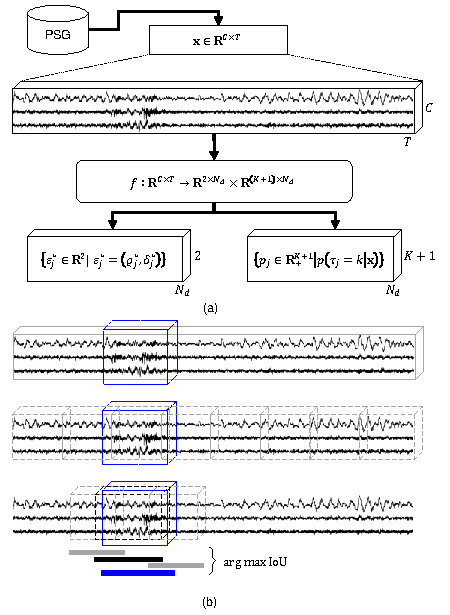
\includegraphics[width=\columnwidth+\marginparwidth+\marginparsep]{figures/paper-iv/embc19-psg_event_detection-fig1-ppt.pdf}
    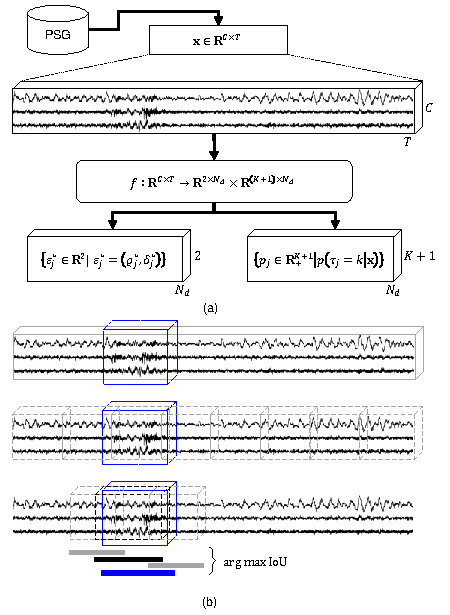
\includegraphics[width=\linewidth]{figures/paper-iv/embc19-psg_event_detection-fig1-ppt.pdf}
    \caption[Event detection schematic]{Schematic of proposed event detection procedure. \textbf{(a)} Input data $\mathbf{x}$ is fed to the model $f$, which outputs predictions for event classes and localizations for each default event in $\varepsilon^{d}$. \textbf{(b)} The IoU for each predicted $\varepsilon^{*}_{j}$ is then calculated with respect to the true event $\varepsilon_{i}$ and non-maximum suppression is applied to match up true events and predictions. In the current case, the predicted event marked in black has the highest IoU with the true event in blue. For more information, see~\cite{Chambon2019,Chambon2018b,Liu2016}.}
    \label{fig:paperiv-schematic}
\end{adjustwidth*}
\end{figure}

\begin{table}
\small
\begin{adjustwidth*}{}{-\marginparwidth-\marginparsep}
\begin{threeparttable}
% \centering
\caption[Event detection network architecture]{Event detection network architecture.}
\label{tab:paperiv-network}
{\footnotesize
\begin{tabular}{@{}lccccccl@{}} \toprule
\textbf{Module}                                                     & \textbf{Input dim.}                                 & \textbf{Output dim.}                                    & \textbf{Type}           & \textbf{Kernel} & \textbf{Filters}                  & \textbf{Stride}      & \textbf{Activation} \\ \midrule
$\phi_{C}$                                                 & $\left(C, T\right)$                        & $\left(C, T\right)$                            & \oned conv & $C$         & $C$                          & 1           & linear \\ \midrule
\multirow[t]{3}{*}{$\phi_{T,\mathrm{init}}$}                  & $\left(C, T\right)$                        & $\left(8, T\right)$                            & \oned conv & $3$         & 8                            & $1$         & -- \\
& $\left(8, T\right)$                        & $\left(8, T\right)$                            & batch norm.    & --          & 8                            & --          & \acs{ReLU} \\
& $\left(8, T\right)$                        & $\left(8, \sfrac{T}{2}\right)$                 & \oned maxpool  & $2$         & --                           & $2$         & -- \\
\multirow[t]{3}{*}{$\phi_{T,n}$} & $\left(2^{n+1}, \sfrac{T}{2^{n-1}}\right)$ & $\left(2^{n+2}, \sfrac{T}{2^{n-1}}\right)$     & \oned conv & $3$         & $2^{n+2}$                    & $1$         & -- \\
& $\left(2^{n+2}, \sfrac{T}{2^{n-1}}\right)$ & $\left(2^{n+2}, \sfrac{T}{2^{n-1}}\right)$     & batch norm.    & --          & $2^{n+2}$                    & --          & \acs{ReLU} \\
& $\left(2^{n+2}, \sfrac{T}{2^{n-1}}\right)$ & $\left(2^{n+2}, \sfrac{T}{2^{n}}\right)$       & \oned maxpool  & $2$         & --                           & $2$         & -- \\ 
\rowcolor{lightlightgray} $\phi_{R}$ & $(\tilde{C}, \tilde{T})$ & $(2\times \tilde{C}, \tilde{T})$ & \acs{bGRU} & $\tilde{C}$ & -- & -- & -- \\ \midrule
$\psi_{\mathrm{clf}}$                                      & $(\tilde{C}, \tilde{T})$                   & $\left( K N_{d}, 1 \right)$ & \oned conv & $\tilde{T}$ & $K N_{d}$ & $\tilde{T}$ & softmax over $K$ filters \\
$\psi_{\mathrm{loc}}$                                      & $(\tilde{C}, \tilde{T})$                   & $\left( 2 N_{d}, 1 \right)$                    & \oned conv & $\tilde{T}$ & $2 N$                        & $\tilde{T}$ & linear \\ \bottomrule
\end{tabular}}
\begin{tablenotes}
\item $\phi_C$, linear mixing module; $\phi_{T}$, temporal feature extraction module; $\phi_{R}$, recurrent neural network module; $\psi_{\mathrm{clf}}$, event classification module; $\psi_{\mathrm{loc}}$, event localization module; $C$, number of input channels; $T$, number of samples in segments; $\tilde{C}=2^{2+n_{\max}}$, number of output channels; $K$, number of event classes; $N_{d}$, number of default events in segment; $\tilde{T}=\sfrac{T}{2^{n_{\max}}}$, reduced temporal dimension; \acs{bGRU}, bidirectional gated recurrent unit; \acs{ReLU}, rectified linear unit.
\end{tablenotes}
\end{threeparttable}
\end{adjustwidth*}
\end{table}

\subsubsection{Network architecture}
The architecture for the proposed \ac{PSG} event detection model closely follows the event detection algorithms described in~\cite{Chambon2018b,Chambon2019}, albeit with some specific changes.
An overview of the proposed network in the model $f$ is provided in~\cref{tab:paperiv-network}.
Briefly, the model comprises three modules:
\begin{enumerate}
\item a channel mixing module $\phi_{C} : \real{C \times T} \to \real{C \times T}$;
\item a feature extraction module $\phi_{T} : \real{C \times T} \to \real{\tilde{C} \times \tilde{T}}$;
\item and an event detection module $\psi$,
\end{enumerate}
the latter contains two submodules performing event classification $\psi_{\mathrm{clf}} : \real{\tilde{C} \times \tilde{T}} \to \real{(K+1)\times N_{d}} $ and event localization $\psi_{\mathrm{loc}} : \real{\tilde{C} \times \tilde{T}} \to \real{2 \times N_{d}}$, respectively.
$\phi_{\mathrm{clf}}$ outputs the probability of the default, non-event class and $K$ event classes, while $\phi_{\mathrm{loc}}$ predicts a start time and a duration of all predicted events relative to a specific default event window.
The channel mixing module $\phi_{C}$ receives a segment of input data $x \in \real{C \times T}$, where $C$ is the number of input channels and $T$ is the number of time samples in the given segment, and subsequently performs linear channel mixing using \oned~convolutions to synthesize $C$ new channels. 
Following $\phi_{C}$, the feature extraction module $\phi_{T}$ consists of $n_{\max}$ blocks with the first block $\phi_{T,1} : \real{C \times T} \to \real{8 \times \sfrac{T}{2}}$ and the $n$th block $\phi_{T,n} : \real{2^{n+1} \times \sfrac{T}{2^{n-1}}} \to \real{2^{k+2} \times \sfrac{T}{2^{n}}}$.
All $n_{\max}$ blocks implement $\phi_{T,n}$ using \oned~convolution layers followed by batch normalization of the feature maps, rectified linear unit activation, and final \oned maximum pooling layers across the temporal dimension.
Kernel sizes and strides for convolution and max. pool. layers in $\phi_{T}$ were set to 3 and 1, and 2 and 2, respectively, while the number of feature maps in $\phi_{T,n}$ was set to $2^{n+2}$.
The event classification submodule $\psi_{\mathrm{clf}}$ is implemented a \oned convolution layer across the entire data volume using $(K+1)N_{d}$ feature maps of size and stride $\tilde{T} = T/2^{n_{\max}}$, where $K \in \mathbf{N}$ is the number of event classes to be detected and $N_{d} \in \mathbf{N}$ is the number of default event windows.
The event localization submodule $\psi_{\mathrm{loc}}$ is likewise implemented using a \oned convolution layer across the entire data volume.

\subsubsection{Data and event sampling}
The proposed network requires an input tensor $x \in \real{C \times T}$ containing \ac{PSG} data in the time segment of size $T$ as well as information about the associated events in the segment.
Since the total number of segments in a standard \ac{PSG} without any event data by far outnumbers the number of segments with event data, we implemented a random sampling of non-event and event classes with the sampling probability of class $k$ inversely proportional to the number of classes, such that $p_k = \frac{1}{K+1},\,k=\left[0\,..\,K \right]$, where $k=0$ is the default (non-event) class.
At training step $t$, we thus sample a class $k$ and afterwards randomly sample a single class $k$ event $\varepsilon_{k}$ between all class $k$ events.
Finally, we extract a segment of \ac{PSG} data of size $C \times T$ with start of segment in the interval $\left[ \bar{\varepsilon}_{k} - T, \bar{\varepsilon}_{k} + T \right]$, where $\bar{\varepsilon}_{k}$ is the sample midpoint of $\varepsilon_{k}$.
This ensures that each $\mathbf{x}$ overlaps 50\% with at least one associated event.

\subsubsection{Optimization of network parameters}
The network parameters were optimized using mini-batch stochastic gradient descent with initial learning rate of \num[retain-unity-mantissa = false]{1e-3} and a momentum of \num{0.9}. 
Mini-batches were balanced with respect to the detected classes. 
The optimization of the network was performed with respect to the same loss function described in~\cite{Chambon2018b,Chambon2019}\graffito{We used a worst negative mining approach with a positive/negative sample ratio of 3.}, and the network was trained until convergence determined by no decrease in the loss on the \eval set over 10 epochs of \train data. 
We also employed learning rate decay with a factor of 2 every 5 epochs of non-decreasing \eval loss.

\subsubsection{Experimental setups}
In this study, we examined two different experimental setups:
\paragraph{Experiment A} First, we investigated the differences in predictive performance using a static vs. a dynamic default event window size. 
This was realized by running six separate training runs with $\tau \in \lbrace \numlist[list-final-separator={, }]{3;5;10;15;20;30} \rbrace \times f_{s}$, as well as a single training run where $f$ was evaluated for all $\tau$ in $\lbrace \numlist[list-final-separator={, }]{3;5;10;15;20;30} \rbrace \times f_{s}$. 
The best performing model was determined by evaluating F1 score on the \eval set for both \ac{LM} and \ac{Ar} detection. 
\paragraph{Experiment B} Second, we tested a network where we added a recurrent processing block $\phi_{R}$ after the feature extraction block $\phi_{T}$ as shown in grey in~\cref{tab:paperiv-network}. 
We considered a single \ac{bGRU} layer with $\tilde{C}$ units. 
Predictions were evaluated across multiple time-scales $\tau \in \lbrace \numlist[list-final-separator={, }]{3;5;10;15} \rbrace \times f_{s}$.

All experiments were implemented in PyTorch 1.0~\cite{Paszke2017,Paszke2019}.

\subsubsection{Performance metrics}
All models were evaluated on the \eval and \test sets using precision (Pr), recall (Re), and F1 scores (F1):
\begin{align}
    \mathrm{Pr} &= \frac{\mathrm{TP}}{\mathrm{TP} + \mathrm{FP}}, \quad \mathrm{Re} = \frac{\mathrm{TP}}{\mathrm{TP} + \mathrm{FN}} \\
    \mathrm{F1} &= 2 \frac{\mathrm{Pr} * \mathrm{Re}}{\mathrm{Pr} + \mathrm{Re}} = \frac{2\mathrm{TP}}{2\mathrm{TP} + \mathrm{FP} + \mathrm{FN}},
\end{align}
where TP, FP, and FN, are the number of true positives, false positives and false negatives, respectively.

% \subsubsection{Statistical analysis}
% Demographic and polysomnographic variables were tested for subset differences with Kruskall-Wallis H-test for independent samples.

\subsection{Results and discussion}
% \newcommand{\fullwidth}{-\marginparwidth-\marginparsep}
\begin{figure}
    % \centering
    \begin{adjustwidth*}{}{-\marginparwidth-\marginparsep}
    \myfloatalign   
    \subfloat[]
    {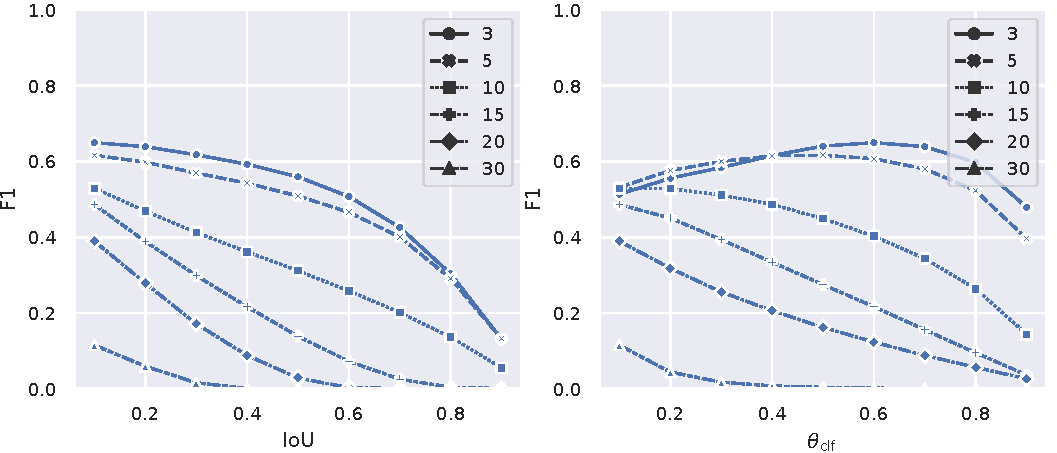
\includegraphics[width=\textwidth]{figures/paper-iv/embc19-mros-limb-default_durations.pdf}\label{fig:paperiv-lm_static}}  \\
    \subfloat[]
    {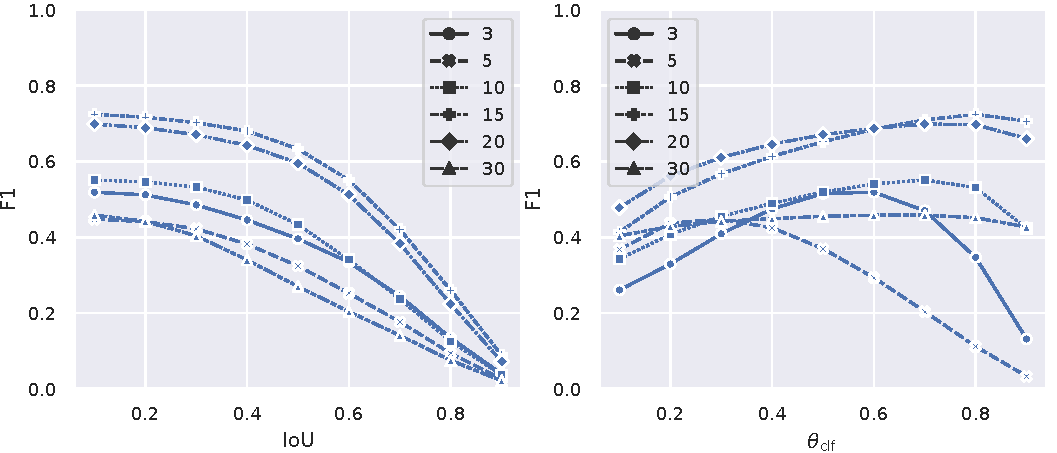
\includegraphics[width=\textwidth]{figures/paper-iv/embc19-arousal-limb-default_durations.pdf}\label{fig:paperiv-ar_static}} \\
    \subfloat[]
    {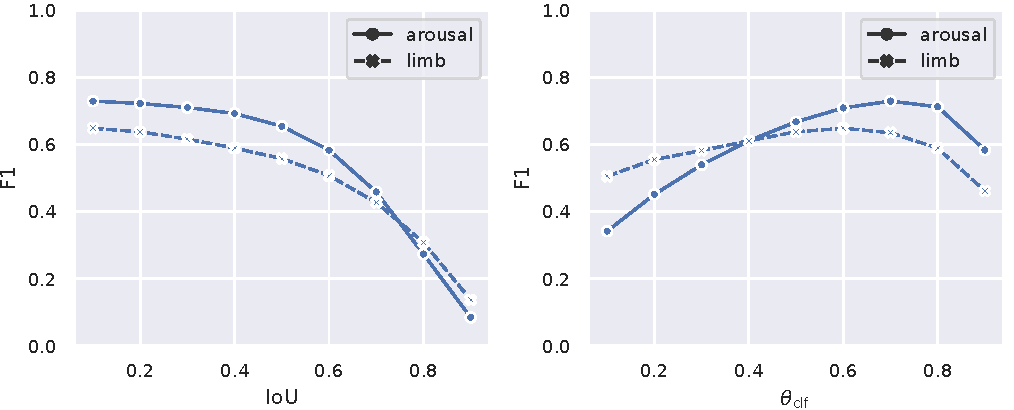
\includegraphics[width=\textwidth]{figures/paper-iv/embc19-mros-arousal_limb-all_durations.pdf}\label{fig:paperiv-ar_lm_dynamic}}
    \caption[Experiment A results]{Experiment A: Optimizing \ac{IoU} and $\theta_{\mathrm{clf}}$ in static models on the \eval set by varying default event window size in seconds in $\lbrace \numlist[list-final-separator={, }]{3;5;10;15;20;30} \rbrace$ \textbf{(a)}-\textbf{(b)}. Left panels show the \ac{IoU} vs. F1 score, while right panels show classification threshold $\theta_{\mathrm{clf}}$ against F1 score. \textbf{(a)} \ac{LM} model. Here, the model performs best for $\mathrm{IoU}=\num{0.1}$ and $\theta_{\mathrm{clf}} = \num{0.6}$ using a window size of $\tau=\SI{3}{\second}\times f_{s}$. \textbf{(b)} \ac{Ar} model. Here, the model performs best for $\ac{IoU}=\num{0.1}$ and $\theta_{\mathrm{clf}} = \num{0.8}$ using a window size of $\tau=\SI{15}{\second} \times f_{s}$. \textbf{(c)} Dynamic models show optimal performance for $\ac{IoU}=\num{0.1}$ and $\theta_{\mathrm{clf}}=\num{0.7}$ and $\theta_{\mathrm{clf}}=\num{0.6}$ for \ac{Ar} and \ac{LM} detection, respectively.}
    \label{fig:paperiv-experiment_a}
    \end{adjustwidth*}
\end{figure}

Shown in~\cref{fig:paperiv-lm_static,fig:paperiv-ar_static} are the F1 scores as a function of \ac{IoU} and the classification threshold $\theta_{\mathrm{clf}}$ for both the \ac{LM} and \ac{Ar} detection models. 
It is apparent that both models perform best with a minimum overlap ($\ac{IoU} = \num{0.1}$) with their respective annotated events, and do not benefit from increasing the overlap. 
This might be caused by the annotated events being imprecise and not by issues with the model itself. 
For example, it is not uncommon to only mark the beginning of an event in standard sleep scoring software, as the duration will automatically be annotated by a default length. \graffito{\SI{3}{\second} for \acp{Ar}, and \SI{0.5}{\second} for \ac{LM} are the minimum durations as defined by \ac{AASM}~\cite{Berry2020}}. 
Future studies will be able to confirm this by either collecting a precisely annotated cohort, or by investigating the average start time and duration discrepancies between annotated and predicted events. 

It is also apparent from~\cref{fig:paperiv-lm_static,fig:paperiv-ar_static} that both detection models benefit from imposing a strict classification threshold. 
Specifically, \ac{LM} detection performance as measured by F1 was highest with $\theta_{\mathrm{clf}} = \num{0.6}$, while maximum \ac{Ar} detection performance was attained with an even higher $\theta_{\mathrm{clf}}$ of \num{0.8}.

By allowing for multiple time-scales in the dynamic models, shown in~\cref{fig:paperiv-ar_lm_dynamic}, we hypothesized that dynamic default event windows would allow for more flexibility and thus better predictive performance. However, we observed no significant differences between the optimal static window and the dynamic window model.

Shown in~\cref{fig:paperiv-experiment_b} are the performance curves for the \ac{RNN} (bidirectional GRU) version of the proposed model for each of the two event detection tasks. 
While the optimal \ac{IoU} and $\theta_{\mathrm{clf}}$ points are unchanged from the static/dynamic models presented in~\cref{fig:paperiv-experiment_a}, the optimal F1 value for \ac{Ar} detection is increased by incorporating temporal dependencies in the model. 
The reverse is true for \ac{LM} detection, which saw a slight decrease in predictive performance caused by lower precision\graffito{See~\cref{tab:paperiv-test_results}}. 
Future work should consider optimizing predictive performance by investigating the effects of varying the number of \ac{bGRU} layers and the number of hidden units in $\phi_{R}$, since this was not performed here.

Application of the optimal models on the \test data is shown in~\cref{tab:paperiv-test_results}. 
With the given architecture of $f$ and the given labels and input data in \train, \ac{LM} detection was maximal for the model with a static/dynamic window, while adding a recurrent module only positively impacted \ac{Ar} prediction. 
Precision and recall decreased for \ac{LM} detection when adding $\phi_{R}$, while precision increased and recall decreased for \ac{Ar} detection. 
An example visualization of the joint distribution of F1 scores obtained from the dynamic model applied to the \test data is shown in~\cref{fig:paperiv-test_distribution}. 
While some outliers are readily observable, especially for \ac{LM} detection, the majority of subject F1 scores follows an approximate bivariate normal distribution.

\begin{figure}
    \centering
    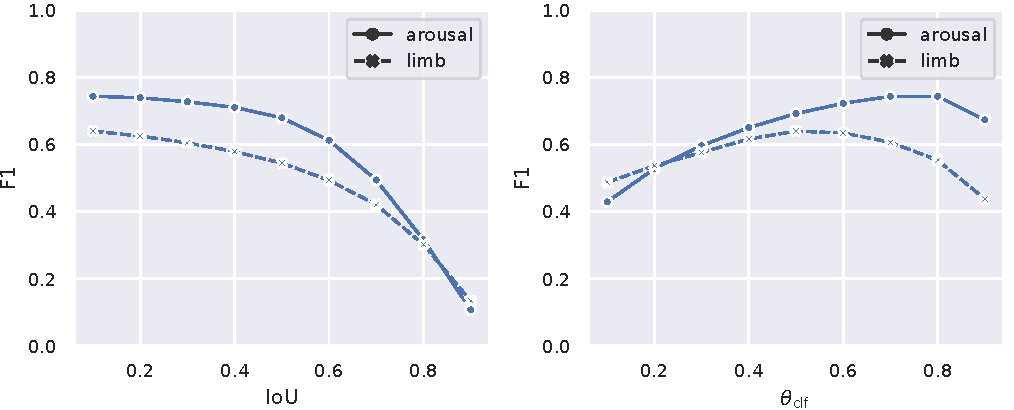
\includegraphics[width=\columnwidth]{figures/paper-iv/embc19-mros-arousal_limb-all_durations_rnn.pdf}
    \caption[Experiment B results]{Experiment B. F1 performance on the \eval set as a function of \ac{IoU} and $\theta_{\mathrm{clf}}$ for \ac{Ar} and \ac{LM} detection when adding the $\phi_{R}$ module. Best performance is seen for $\ac{IoU}=\num{0.1}$ for both \ac{Ar} and \ac{LM} detection, and $\theta_{\mathrm{clf}} = \num{0.6}$ and $\theta_{\mathrm{clf}}=\num{0.8}$ for \ac{LM} and \ac{Ar} detection, respectively.}
    \label{fig:paperiv-experiment_b}
\end{figure}

Subset partitions were reasonably well-distributed with no significant differences between key variables, see~\cref{tab:paperiv-demographics}. 
An exception is the \ac{AHI}, although the associated effect is small and most likely a result of the low sample size in \eval compared to \train and \test. 
It is noted, that although \ac{AHI}, \ac{ArI}, and \ac{PLMI} are not normally distributed and summarizing these variables with standard deviations is invalid, it is nevertheless standard practice in sleep medicine and thus presented the same way here. 
We performed little data cleaning in order to provide as much data and variation to the deep learning model as possible, however, future efforts should explore and apply inclusion criteria such as minimal total sleep time, artifact detection and removal of studies with severe artifacts. 
We did impose a trivial lower bound on the number of scored events (\num{>0}) for a \ac{PSG} to be included in this study, but stricter requirements could potentially improve model performance.
\begin{figure}[t]
    \centering
    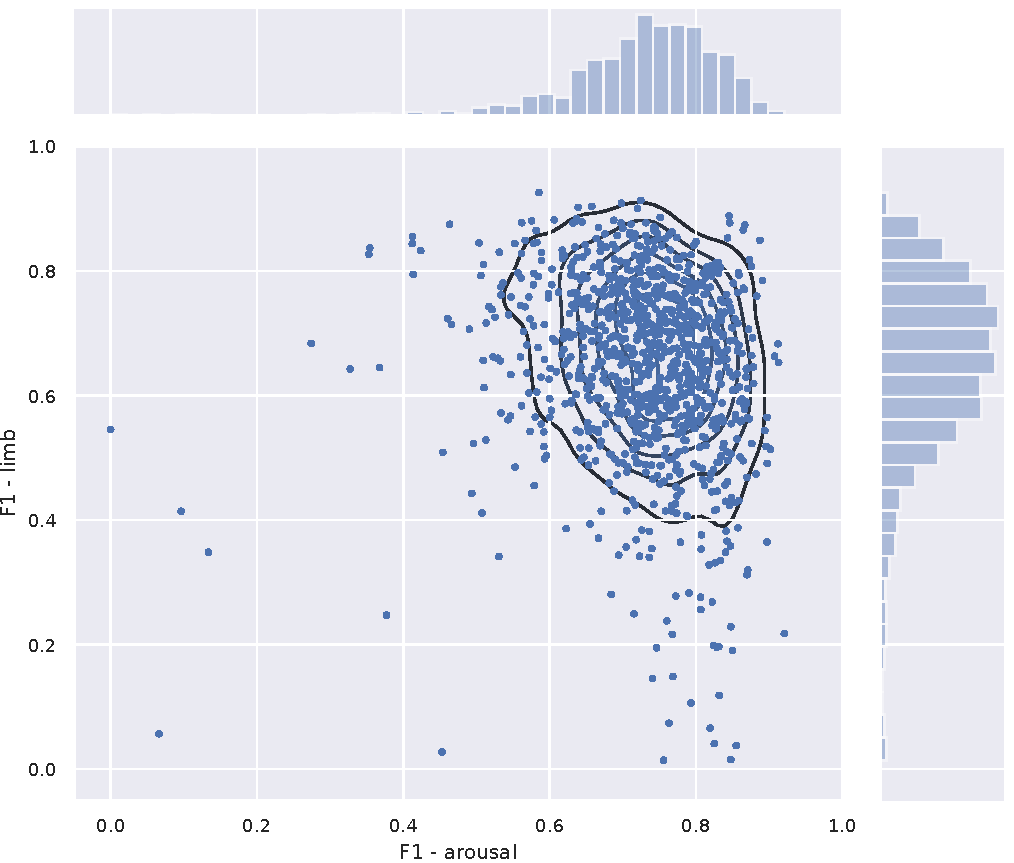
\includegraphics[width=\textwidth]{figures/paper-iv/embc19-distribution.pdf}
    \caption[Visualization of F1 scores]{Visualization of F1 scores for both \ac{Ar} and \ac{LM} detection using the dynamic model.}
    \label{fig:paperiv-test_distribution}
\end{figure}
\begin{table}[tb]
    \sisetup{separate-uncertainty}
    \small
    \centering
    \begin{threeparttable}
    \caption[Optimized test performance]{Application of optimized models on \test data.}
    \label{tab:paperiv-test_results}
    \begin{tabular}{@{}lSSS@{}} \toprule
        \textbf{Model} & \textbf{F1} & \textbf{Pr} & \textbf{Re} \\ \midrule
        \ac{LM}, static & \num{0.648 \pm 0.148} & \num{0.631 \pm 0.181} & \num{0.720 \pm 0.141} \\
        \ac{Ar}, static & \num{0.727 \pm 0.102} & \num{0.706 \pm 0.113} & \num{0.771 \pm 0.132} \\
        \ac{LM}, dynamic & \num{0.647 \pm 0.148} & \num{0.627 \pm 0.181} & \num{0.722 \pm 0.14} \\
        \ac{Ar}, dynamic. & \num{0.729 \pm 0.102} & \num{0.699 \pm 0.115} & \num{0.785 \pm 0.131} \\ \midrule
        \ac{LM}, \ac{RNN} & \num{0.639 \pm 0.147} & \num{0.606 \pm 0.180} & \num{0.727 \pm 0.126} \\
        \ac{Ar}, \ac{RNN} & \num{0.749 \pm 0.105} & \num{0.772 \pm 0.107} & \num{0.748 \pm 0.138} \\ \bottomrule
    \end{tabular}
    \begin{tablenotes}
    \item Data are shown as subject-averaged F1, precision (Pr) and recall (Re) with associated standard deviations. Top four rows correspond to Experiment A, while bottom two rows correspond to Experiment B. \ac{Ar}: arousal; \ac{LM}: leg movement; \ac{RNN}: recurrent neural network.
    \end{tablenotes}
    \end{threeparttable}
\end{table}
In this work, we investigated somatic \ac{PSG} events present in multiple signal modalities instead of \ac{EEG}-specific events, which required changes to the network architecture. 
Specifically, we kept the signal modality encoded in the first dimension of the tensor propagated through the network, which allowed for the use of \oned convolutional operators. 
By performing \oned convolutions and keeping the channel information in the feature maps instead of keeping them as separate dimensions and performing \twod convolutions as proposed in~\cite{Chambon2018b,Chambon2019}, we simplify and reduce the number of computations and training time by a factor $\propto C$. 

However, we did not investigate the effects of modeling the conditional probability of \ac{Ar} and \ac{LM} occurrence, but the proposed architecture is versatile enough to detect both events jointly as well as separately. 
Previous work also suggest that detecting multiple objects at the same time is of high interest and leads to (at least) non-inferior performances~\cite{Chambon2018b, Chambon2019, Redmon2016a, Redmon2016b, Liu2016}.

Additionally, we speculated that the temporal dynamics of the \ac{PSG} signals were important for optimal event detection performance. 
Although the effects were small, the F1 score in \ac{Ar} detection increased when adding an \ac{RNN} module to the network before the detection module. 
However, this was not the case for \ac{LM} detection, which is most likely due to the different temporal and physiological characteristics of the two events in question. 

Future efforts will address the fact that events are mutually exclusive in the current modeling scheme, given a certain default event window size. 
However, it is common to see \acp{Ar} and \acp{LM} as a result of one another, and thus, if the window size is too small, a more unlikely event, as measured by classification threshold and \ac{IoU}, will be removed even if it matches up to a specific true event of a certain class. 